To safe power with an conventional receiver, it needs to be programmed in such a way, that the microcontroller is kept in a low power sleep mode.
To check for if any data was sent, it needs to wake up periodically to check for notifications.
To set this period is a trade off between response time and power consumption.
Is the period larger, the receiver is a longer time in its low power mode.
But this period on the other side defines directly the response time, since data can only be received in the wake up mode.

\begin{figure}[h]
	\centering
	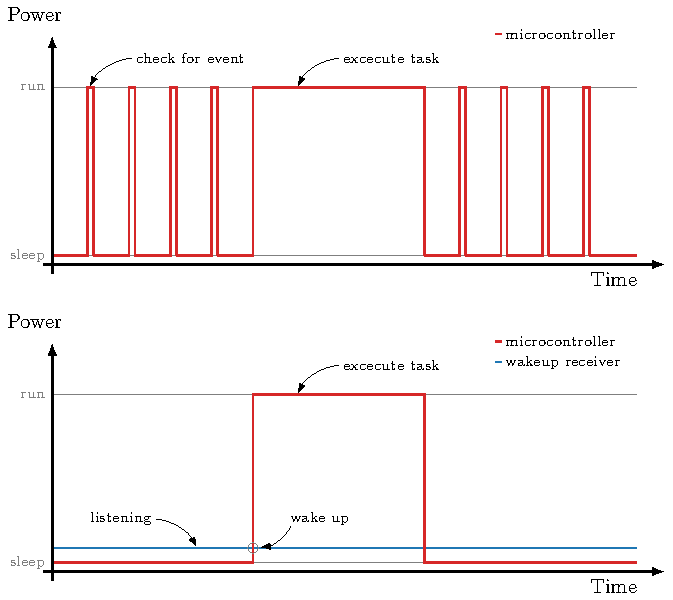
\includegraphics[width=0.9\textwidth]{2-theory/wakeup/graphics/wake_comp.pdf}
	\caption{Microcontroller checks periodically for incoming data (top), wakeup receiver is constantly listening (bottom)\label{theory:wake}}
\end{figure}
xxx
A wakeup receiver now allows a device to be constantly in listening mode, while consuming low energy.
Added to the system, the actual wireless module, over which the data later is transmitted stays shut down and only the wakeup receiver is listening.
After receiving a defined pattern over this channel, the wakeup receiver generates an interrupt to wake up the microcontroller. 
it can now establish a channel over a different wireless module, or execute another task.
When done, the microcontroller puts itself and all other modules in sleep mode again.
